\documentclass[tikz,border=5pt]{standalone}
\usepackage{tikz}
\usetikzlibrary{arrows.meta,decorations.markings,calc}

\begin{document}

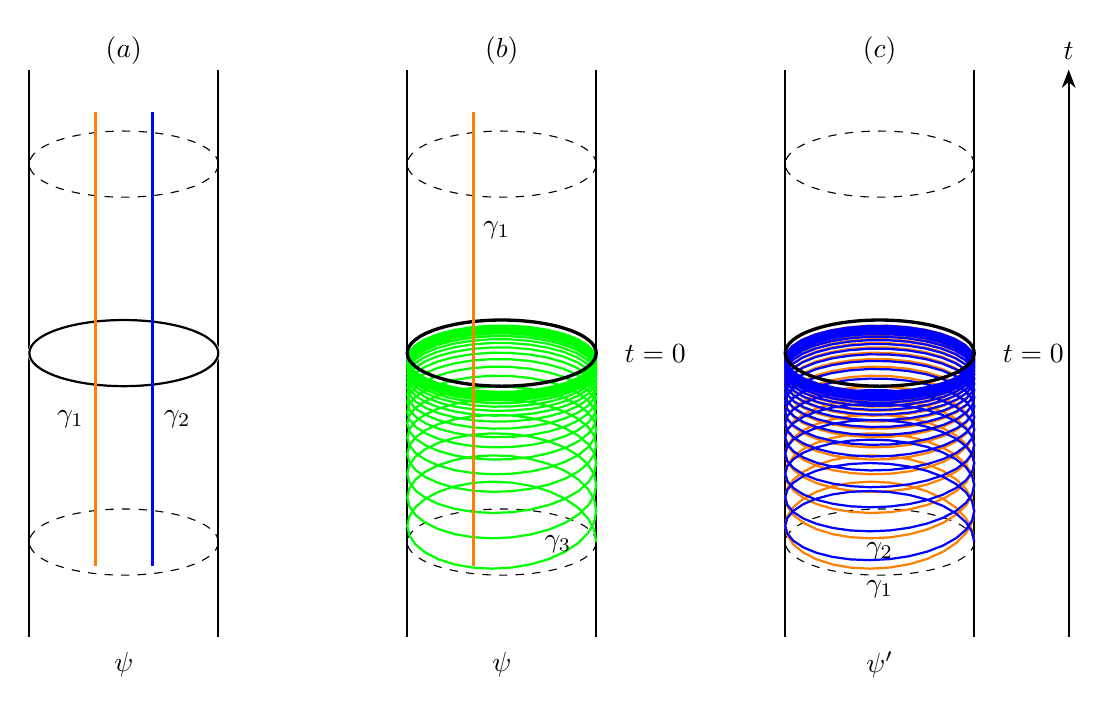
\begin{tikzpicture}[>=Stealth,scale=1.2]

% ---------------- RIGHT CYLINDER ----------------
\begin{scope}[shift={(4,0)}]

% cylinder sides
\draw[thick] (-1,-3) -- (-1,3);
\draw[thick] (1,-3) -- (1,3);

% top and bottom ellipses (dashed)
\draw[dashed] (0,2) ellipse (1 and 0.35);
\draw[dashed] (0,0) ellipse (1 and 0.35);
\draw[dashed] (0,-2) ellipse (1 and 0.35);

% vertical time arrow
%\draw[red,thick,->] (0,-3) -- (0,3) node[above] {$\tilde r_{-}$};

% Spiral on cylinder surface: use 3D->2D projection
% param t \in [0,4], theta = omega * t (radians)
% r(t) -> 1, z(t) -> 0 as t increases
%\draw[blue,thick,->,samples=600,variable=\t,domain=0:4]
 %plot ({ (1 + 0.0*exp(-1.2*\t))*cos(8*pi*\t r) },
       %{ 2*exp(-1.0*\t) + 0.35*(1 + 0.6*exp(-1.6*\t))*sin(8*pi*\t r) } );

\draw[orange,thick,->,samples=600,variable=\t,domain=0:4]
 plot ({ (1 + 0.0*exp(-1.0*\t))*cos(10*pi*\t r) },
       { -2*exp(-0.9*\t) + 0.35*(1 + 0.6*exp(-1.0*\t))*sin(10*pi*\t r) } );

\draw[blue,thick,->,samples=600,variable=\t,domain=0:4]
 plot ({ (1 + 0.0*exp(-1.0*\t))*cos(10*pi*\t r) },
       { -2*exp(-0.9*\t) + 0.35*(1 + 0.3*exp(-1.0*\t))*sin(10*pi*\t r) } );

% overlay the compactified circle (solid) at z=0
\draw[black,very thick] (0,0) ellipse (1 and 0.35);

\node[right] at (1.2,0) {$t=0$};
%\node at (6.5,0.0) { $t=0$ };

% rotation arrow
%\draw[->] (-0.5,-3.3) arc (200:340:0.7);
\node at (0.0,-3.3) {$\psi'$};
\node at (0.0,3.2) {$(c)$};

\node at (-0.0,-2.1) {$\gamma_2$};
\node at (0.0,-2.5) {$\gamma_1$};

\end{scope}

% ---------------- MIDDLE CYLINDER ----------------
\begin{scope}[shift={(0,0)}]

% cylinder sides
\draw[thick] (-1,-3) -- (-1,3);
\draw[thick] (1,-3) -- (1,3);

% top and bottom ellipses (dashed)
\draw[dashed] (0,2) ellipse (1 and 0.35);
\draw[dashed] (0,0) ellipse (1 and 0.35);
\draw[dashed] (0,-2) ellipse (1 and 0.35);

% vertical time arrow
%\draw[red,thick,->] (0,-3) -- (0,3) node[above] {$\tilde r_{-}$};

% Spiral on cylinder surface: use 3D->2D projection
% param t \in [0,4], theta = omega * t (radians)
% r(t) -> 1, z(t) -> 0 as t increases
%\draw[blue,thick,->,samples=600,variable=\t,domain=0:4]
 %plot ({ (1 + 0.0*exp(-1.2*\t))*cos(8*pi*\t r) },
       %{ 2*exp(-1.0*\t) + 0.35*(1 + 0.6*exp(-1.6*\t))*sin(8*pi*\t r) } );
\draw[green,thick,->,samples=600,variable=\t,domain=0:4]
 plot ({ (1 + 0.0*exp(-1.0*\t))*cos(10*pi*\t r) },
       { -2*exp(-0.9*\t) + 0.35*(1 + 0.6*exp(-1.0*\t))*sin(10*pi*\t r) } );

% overlay the compactified circle (solid) at z=0
\draw[black,very thick] (0,0) ellipse (1 and 0.35);

\node[right] at (1.2,0) {$t=0$};
%\node at (6.5,0.0) { $t=0$ };

% rotation arrow
%\draw[->] (-0.5,-3.3) arc (200:340:0.7);
\node at (0.0,-3.3) {$\psi$};
\node at (0.0,3.2) {$(b)$};
\node[right] at (0.35,-2.02) {$\gamma_3$};
\node[right] at (-0.3,1.3) {$\gamma_1$};

\end{scope}


% ---------------- CENTRAL Z AXIS ----------------
\draw[thick,->] (6,-3) -- (6,3) node[above] {$t$};


% ---------------- LEFT CYLINDER ----------------
\begin{scope}[shift={(-4,0)}]

% cylinder sides
\draw[thick] (-1,-3) -- (-1,3);
\draw[thick] (1,-3) -- (1,3);

% slices (dashed)
\draw[dashed] (0,2) ellipse (1 and 0.35);
\draw[dashed] (0,0) ellipse (1 and 0.35);
\draw[dashed] (0,-2) ellipse (1 and 0.35);

% vertical arrow
%\draw[green!70!black,thick,->] (0,-3) -- (0,3) node[above] {$\tilde r_{+}$};

% Spiral from below approaching z=0 (same projection rule)


% overlay the compactified circle (solid) at z=0
\draw[white,very thick] (0,0) ellipse (1 and 0.35);

% middle slice
\draw[thick] (0,0) ellipse (1 and 0.35);
\node at (0.0,-3.3) {$\psi$};
\node at (0.0,3.2) {$(a)$};
% rotation arrow
%\draw[->] (-0.5,-3.3) arc (200:340:0.7);

%\draw[->,thick,red] (-2.0 cm, -3-0.4) -- ++(0, 6 + 0.8) node[midway,right] {$t$};
%\draw[-,line width=1.0pt,blue] (3.75 cm, -3 + 0.75) -- ++(0, 6 - 1.2) ;
\draw[-,line width=1.0pt,blue] (0.3 cm, -3 + 0.75) -- ++(0, 6 - 1.2) ;
\draw[-,line width=1.0pt,orange] (-0.3 cm, -3 + 0.75) -- ++(0, 6 - 1.2) ;
\draw[-,line width=1.0pt,orange] (3.7 cm, -3 + 0.75) -- ++(0, 6 - 1.2);
% -------------------------

%\begin{scope}
  %\draw[black!60,dashed] (-1.8,0) ellipse (0.95 and 0.18);
  %\draw[black!60] (1.8,1.6) ellipse (1.15 and 0.2);
  
  %\node at (1.8,0.0) { $t=0$ };
%\end{scope}

% -------------------------
% Example labels near curves (tweak positions as needed)
% -------------------------
%\node[right] at (-4.0,-1.25){$\gamma_1$};
\node[left] at (-0.32,-0.7) {$\gamma_1$};
\node[right] at (0.32,-0.7) {$\gamma_2$};


\end{scope}

\end{tikzpicture}

\end{document}